\documentclass[a4paper]{article}

\input{style/ch_xelatex.tex}
\input{style/scala.tex}

%代码段设置
\lstset{numbers=left,
basicstyle=\tiny,
numberstyle=\tiny,
keywordstyle=\color{blue!70},
commentstyle=\color{red!50!green!50!blue!50},
frame=single, rulesepcolor=\color{red!20!green!20!blue!20},
escapeinside=``
}

\graphicspath{ {images/} }
\usepackage{ctex}
\usepackage{graphicx}
\usepackage{color,framed}%文本框
\usepackage{listings}
\usepackage{caption}
\usepackage{amssymb}
\usepackage{enumerate}
\usepackage{xcolor}
\usepackage{bm} 
\usepackage{lastpage}%获得总页数
\usepackage{fancyhdr}
\usepackage{tabularx}  
\usepackage{geometry}
\usepackage{minted}
\usepackage{graphics}
\usepackage{subfigure}
\usepackage{float}
\usepackage{pdfpages}
\usepackage{pgfplots}
\pgfplotsset{width=10cm,compat=1.9}
\usepackage{multirow}
\usepackage{footnote}
\usepackage{booktabs}

%-----------------------伪代码------------------
\usepackage{algorithm}  
\usepackage{algorithmicx}  
\usepackage{algpseudocode}  
\floatname{algorithm}{Algorithm}  
\renewcommand{\algorithmicrequire}{\textbf{Input:}}  
\renewcommand{\algorithmicensure}{\textbf{Output:}} 
\usepackage{lipsum}  
\makeatletter
\newenvironment{breakablealgorithm}
  {% \begin{breakablealgorithm}
  \begin{center}
     \refstepcounter{algorithm}% New algorithm
     \hrule height.8pt depth0pt \kern2pt% \@fs@pre for \@fs@ruled
     \renewcommand{\caption}[2][\relax]{% Make a new \caption
      {\raggedright\textbf{\ALG@name~\thealgorithm} ##2\par}%
      \ifx\relax##1\relax % #1 is \relax
         \addcontentsline{loa}{algorithm}{\protect\numberline{\thealgorithm}##2}%
      \else % #1 is not \relax
         \addcontentsline{loa}{algorithm}{\protect\numberline{\thealgorithm}##1}%
      \fi
      \kern2pt\hrule\kern2pt
     }
  }{% \end{breakablealgorithm}
     \kern2pt\hrule\relax% \@fs@post for \@fs@ruled
  \end{center}
  }
\makeatother
%------------------------代码-------------------
\usepackage{xcolor} 
\usepackage{listings} 
\lstset{ 
breaklines,%自动换行
basicstyle=\small,
escapeinside=``,
keywordstyle=\color{ blue!70} \bfseries,
commentstyle=\color{red!50!green!50!blue!50},% 
stringstyle=\ttfamily,% 
extendedchars=false,% 
linewidth=\textwidth,% 
numbers=left,% 
numberstyle=\tiny \color{blue!50},% 
frame=trbl% 
rulesepcolor= \color{ red!20!green!20!blue!20} 
}

%-------------------------页面边距--------------
\geometry{a4paper,left=2.3cm,right=2.3cm,top=2.7cm,bottom=2.7cm}
%-------------------------页眉页脚--------------
\usepackage{fancyhdr}
\pagestyle{fancy}
\lhead{\kaishu \leftmark}
% \chead{}
\rhead{\kaishu 深度学习进阶课 实验报告}%加粗\bfseries 
\lfoot{}
\cfoot{\thepage}
\rfoot{}
\renewcommand{\headrulewidth}{0.1pt}  
\renewcommand{\footrulewidth}{0pt}%去掉横线
\newcommand{\HRule}{\rule{\linewidth}{0.5mm}}%标题横线
\newcommand{\HRulegrossa}{\rule{\linewidth}{1.2mm}}
\setlength{\textfloatsep}{10mm}%设置图片的前后间距
%--------------------文档内容--------------------

\begin{document}
\renewcommand{\contentsname}{目\ 录}
\renewcommand{\appendixname}{附录}
\renewcommand{\appendixpagename}{附录}
\renewcommand{\refname}{参考文献} 
\renewcommand{\figurename}{图}
\renewcommand{\tablename}{表}
\renewcommand{\today}{\number\year 年 \number\month 月 \number\day 日}

%-------------------------封面----------------
\begin{titlepage}
    \begin{center}
    \includegraphics[width=0.8\textwidth]{NKU.png}\\[1cm]
    \vspace{20mm}
		\textbf{\huge\textbf{\kaishu{计算机学院}}}\\[0.5cm]
		\textbf{\huge{\kaishu{深度学习及应用（高阶课） 实验报告}}}\\[2.3cm]
		\textbf{\Huge\textbf{\kaishu{卷积神经网络算法}}}

		\vspace{\fill}
    
    % \textbf{\Large \textbf{并行程序设计期末实验报告}}\\[0.8cm]
    % \HRule \\[0.9cm]
    % \HRule \\[2.0cm]
    \centering
    \textsc{\LARGE \kaishu{姓名\ :\ 申健强}}\\[0.5cm]
    \textsc{\LARGE \kaishu{学号\ :\ 2313119}}\\[0.5cm]
    \textsc{\LARGE \kaishu{专业\ :\ 计算机科学与技术}}\\[0.5cm]
    
    \vfill
    {\Large \today}
    \end{center}
\end{titlepage}

\renewcommand {\thefigure}{\thesection{}.\arabic{figure}}%图片按章标号
\renewcommand{\figurename}{图}
\renewcommand{\contentsname}{目录}  
\cfoot{\thepage\ of \pageref{LastPage}}%当前页 of 总页数


% 生成目录
\clearpage
\tableofcontents
\newpage
%-------------------- 正文 --------------------
\section{实验目的与要求}
本实验的目标是掌握卷积神经网络（CNN）的基本原理，并使用 PyTorch 在 CIFAR-10 数据集上完成以下工作：
\begin{itemize}
  \item 复现老师提供的原始版本 CNN，给出网络结构与在测试集上的损失、准确率曲线；
  \item 自行实现 \textbf{ResNet}、\textbf{DenseNet}、\textbf{MobileNet} 三种网络并完成同样的训练与评测；
  \item 重点分析\textbf{无跳跃连接的 CNN、ResNet、DenseNet、MobileNet 在训练过程中的差异}；
  \item 扩展部分实现 \textbf{Res2Net}，并通过实验说明其相对前述网络的优势与劣势。
\end{itemize}

\section{数据集与统一训练协议}
\textbf{数据集.} CIFAR-10 包含 10 类共 60{,}000 张 $32\times32$ 彩色图像，其中训练集 50{,}000 张、测试集 10{,}000 张。由于 CIFAR-10 未单独划分验证集，本实验沿用惯例，以 10{,}000 张测试集作为验证/评测集，后文“验证集曲线”即在该集合上得到。训练集采用标准数据增强：\texttt{RandomCrop(32, padding=4)} 与 \texttt{RandomHorizontalFlip}；训练、测试均按 CIFAR-10 的通道均值 $(0.4914,0.4822,0.4465)$、标准差 $(0.2470,0.2435,0.2616)$ 归一化。

\textbf{训练协议.} 为保证五个模型可公平对比，全部采用\textbf{相同}的训练设置：优化器 SGD（动量 $0.9$，权重衰减 $5\times10^{-4}$），学习率 $0.01$，损失函数为交叉熵，批大小 128，训练 30 个 epoch，固定随机种子 42。训练循环沿用老师给出的标准写法（前向 $\rightarrow$ 计算损失 $\rightarrow$ 反向 $\rightarrow$ 更新），并在每个 epoch 结束后在测试集上评估一次，记录损失与 Top-1 准确率以绘制曲线。代码结构上，五个模型统一定义在 \texttt{models.py}，数据/训练/评估工具在 \texttt{train\_utils.py}，可视化与对比在 notebook 中完成。

\textbf{实验环境.} PyTorch + 单张 NVIDIA GPU（CUDA）。

\section{各模型结构与原理}
五个网络的结构概览见表~\ref{tab:arch}。除基线 CNN 外，其余网络均使用 $3\times3$ 卷积作为 CIFAR 适配的 stem（步长 1、不接 maxpool，以免在 $32\times32$ 的小图上过早下采样），分类头前统一使用全局平均池化。

\begin{table}[H]
  \centering
  \caption{五个模型的结构概览}
  \label{tab:arch}
  \begin{tabular}{lllr}
    \toprule
    模型 & 主体结构 & 核心思想 & 参数量 \\
    \midrule
    BaselineCNN & 2 个卷积 + 3 个全连接 & 无跳跃连接（对照基线） & 0.062\,M \\
    ResNet18    & 4 stage $\times$ 2 BasicBlock & 残差连接 $y=F(x)+x$ & 11.17\,M \\
    DenseNet    & 4 DenseBlock(6) + 3 Transition, $k{=}12$ & 密集连接（特征拼接复用） & 0.246\,M \\
    MobileNet   & 13 个深度可分离卷积块 & 深度可分离卷积（轻量化） & 3.22\,M \\
    Res2Net     & 4 stage $\times$ 2 Bottle2neck, $scale{=}4$ & 块内多尺度分组残差 & 13.84\,M \\
    \bottomrule
  \end{tabular}
\end{table}

\subsection{Baseline CNN}
该网络为最朴素的卷积结构，无批归一化、无跳跃连接，结构如下：
\begin{lstlisting}
class Net(nn.Module):
    def __init__(self):
        super().__init__()
        self.conv1 = nn.Conv2d(3, 6, 5)
        self.pool  = nn.MaxPool2d(2, 2)
        self.conv2 = nn.Conv2d(6, 16, 5)
        self.fc1   = nn.Linear(16 * 5 * 5, 120)
        self.fc2   = nn.Linear(120, 84)
        self.fc3   = nn.Linear(84, 10)
    def forward(self, x):
        x = self.pool(F.relu(self.conv1(x)))
        x = self.pool(F.relu(self.conv2(x)))
        x = torch.flatten(x, 1)
        x = F.relu(self.fc1(x)); x = F.relu(self.fc2(x))
        return self.fc3(x)
\end{lstlisting}

\subsection{ResNet}
ResNet 通过\textbf{残差连接}让每个模块学习残差映射并与输入做恒等相加：
\begin{equation}
  \bm{y} = \mathcal{F}(\bm{x}, \{W_i\}) + \bm{x},
\end{equation}
恒等捷径为梯度提供了“直通路径”，缓解了深层网络的梯度消失与退化问题，使网络能够稳定地加深。本实验采用 CIFAR 版 ResNet-18（BasicBlock，含 BatchNorm；stem 为 $3\times3$ 卷积，4 个 stage 通道数 $64\!\to\!128\!\to\!256\!\to\!512$，每 stage 2 个 BasicBlock）。核心残差模块实现如下：
\begin{lstlisting}
class BasicBlock(nn.Module):                 # expansion = 1
    def __init__(self, in_planes, planes, stride=1):
        super().__init__()
        self.conv1 = nn.Conv2d(in_planes, planes, 3, stride, 1, bias=False)
        self.bn1   = nn.BatchNorm2d(planes)
        self.conv2 = nn.Conv2d(planes, planes, 3, 1, 1, bias=False)
        self.bn2   = nn.BatchNorm2d(planes)
        self.shortcut = nn.Sequential()       # 1x1 conv to align dims if needed
        if stride != 1 or in_planes != planes:
            self.shortcut = nn.Sequential(
                nn.Conv2d(in_planes, planes, 1, stride, bias=False),
                nn.BatchNorm2d(planes))
    def forward(self, x):
        out = F.relu(self.bn1(self.conv1(x)))
        out = self.bn2(self.conv2(out))
        out += self.shortcut(x)               # residual add
        return F.relu(out)
\end{lstlisting}

\subsection{DenseNet}
DenseNet 将每一层与其之前\textbf{所有层}在通道维拼接，第 $l$ 层的输入为
\begin{equation}
  \bm{x}_l = H_l\!\left([\bm{x}_0, \bm{x}_1, \dots, \bm{x}_{l-1}]\right).
\end{equation}
这种密集连接带来强烈的\textbf{特征复用}，使其能以极少的参数达到较高精度；每层都能直接获得来自损失的梯度，梯度流动顺畅。本实验使用 DenseNet-BC（增长率 $k=12$，4 个 DenseBlock 各 6 层，块间以 Transition 层做 $1\times1$ 卷积压缩 + 平均池化下采样）。稠密层与过渡层实现如下：
\begin{lstlisting}
class _DenseBottleneck(nn.Module):            # concat output with input
    def __init__(self, in_planes, k):
        super().__init__()
        self.bn1 = nn.BatchNorm2d(in_planes)
        self.conv1 = nn.Conv2d(in_planes, 4*k, 1, bias=False)
        self.bn2 = nn.BatchNorm2d(4*k)
        self.conv2 = nn.Conv2d(4*k, k, 3, padding=1, bias=False)
    def forward(self, x):
        out = self.conv1(F.relu(self.bn1(x)))
        out = self.conv2(F.relu(self.bn2(out)))
        return torch.cat([out, x], 1)         # dense concat

class _Transition(nn.Module):                 # compress channels + downsample
    def __init__(self, in_planes, out_planes):
        super().__init__()
        self.bn = nn.BatchNorm2d(in_planes)
        self.conv = nn.Conv2d(in_planes, out_planes, 1, bias=False)
    def forward(self, x):
        return F.avg_pool2d(self.conv(F.relu(self.bn(x))), 2)
\end{lstlisting}

\subsection{MobileNet}
MobileNet 用\textbf{深度可分离卷积}替代标准卷积：先逐通道（depthwise）$3\times3$ 卷积，再用 $1\times1$（pointwise）卷积融合通道。相比标准卷积，计算量从 $D_K^2\cdot M\cdot N\cdot D_F^2$ 降为 $D_K^2\cdot M\cdot D_F^2 + M\cdot N\cdot D_F^2$，大幅减少参数与计算量，是轻量化网络的代表。本实验堆叠 13 个深度可分离卷积块（通道按 $64,128,128,256,256,512\!\times\!6,1024,1024$ 递增，其中 4 处用 stride 2 下采样），核心模块实现如下：
\begin{lstlisting}
class _DepthwiseSeparable(nn.Module):
    def __init__(self, in_planes, out_planes, stride=1):
        super().__init__()
        # depthwise conv (groups=in_planes), per-channel
        self.conv1 = nn.Conv2d(in_planes, in_planes, 3, stride, 1,
                               groups=in_planes, bias=False)
        self.bn1 = nn.BatchNorm2d(in_planes)
        # pointwise 1x1 conv, fuse channels
        self.conv2 = nn.Conv2d(in_planes, out_planes, 1, bias=False)
        self.bn2 = nn.BatchNorm2d(out_planes)
    def forward(self, x):
        out = F.relu(self.bn1(self.conv1(x)))
        return F.relu(self.bn2(self.conv2(out)))
\end{lstlisting}

\subsection{Res2Net}
Res2Net 在 bottleneck 内部将通道划分为 $scale$ 组，组间做\textbf{层级残差}：
\begin{equation}
  \bm{y}_i =
  \begin{cases}
    \bm{x}_i, & i=1\\
    K_i(\bm{x}_i + \bm{y}_{i-1}), & 1<i\le scale
  \end{cases}
\end{equation}
由此在\textbf{单个模块内}获得多种感受野尺度的组合，增强了多尺度特征表达能力。本实验使用 $scale=4$、$baseWidth=26$ 的 Bottle2neck，骨架与 ResNet 一致（4 个 stage，每 stage 2 个 Bottle2neck，expansion$=4$）。其前向中的多尺度分组残差实现如下：
\begin{lstlisting}
def forward(self, x):                          # Bottle2neck, scale=4
    residual = x
    out = self.relu(self.bn1(self.conv1(x)))
    spx = torch.split(out, self.width, 1)      # split channels into scale groups
    for i in range(self.nums):
        sp = spx[i] if (i == 0 or self.stype == 'stage') else sp + spx[i]
        sp = self.relu(self.bns[i](self.convs[i](sp)))   # hierarchical residual
        out = sp if i == 0 else torch.cat((out, sp), 1)
    if self.scale != 1:                        # concat the last group
        out = torch.cat((out, spx[self.nums]), 1)
    out = self.bn3(self.conv3(out))
    if self.downsample is not None:
        residual = self.downsample(x)
    return self.relu(out + residual)
\end{lstlisting}

\section{实验结果}
五个模型在统一协议下训练 30 个 epoch，总体结果见表~\ref{tab:result}。为便于横向对比，各模型的损失曲线、准确率曲线均绘于同一坐标系并以颜色与图例区分，故 CNN、ResNet、DenseNet、MobileNet、Res2Net 各自的训练/验证曲线均可在图~\ref{fig:loss} 与图~\ref{fig:acc} 中直接读出。

\begin{table}[H]
  \centering
  \caption{各模型总体结果对比}
  \label{tab:result}
  \begin{tabular}{lrrrr}
    \toprule
    模型 & 参数量(M) & 最佳准确率(\%) & 最终准确率(\%) & 训练耗时(min) \\
    \midrule
    BaselineCNN & 0.062  & 68.72 & 67.17 & 13.3 \\
    ResNet18    & 11.17  & 89.82 & 89.82 & 21.9 \\
    DenseNet    & 0.246  & 87.38 & 86.64 & 20.4 \\
    MobileNet   & 3.22   & 84.60 & 83.83 & 12.7 \\
    Res2Net     & 13.84  & \textbf{89.92} & \textbf{89.92} & 45.5 \\
    \bottomrule
  \end{tabular}
\end{table}

\textbf{损失曲线.} 图~\ref{fig:loss} 给出训练集与测试集的损失随 epoch 的变化。带跳跃/密集连接并使用 BatchNorm 的四个网络损失下降明显快于基线 CNN，其中 ResNet 与 Res2Net 的训练损失最低。

\begin{figure}[H]
  \centering
  \includegraphics[width=\textwidth]{fig_loss.png}
  \caption{训练集（左）与测试集（右）损失曲线}
  \label{fig:loss}
\end{figure}

\textbf{准确率曲线.} 图~\ref{fig:acc} 显示测试集 Top-1 准确率。ResNet/Res2Net 收敛最快、最终最高；DenseNet 次之但仅用 0.25\,M 参数；MobileNet 略低；基线 CNN 始终最低，约 68\%。

\begin{figure}[H]
  \centering
  \includegraphics[width=0.72\textwidth]{fig_acc.png}
  \caption{测试集准确率随 epoch 的变化}
  \label{fig:acc}
\end{figure}

\textbf{准确率与参数量.} 图~\ref{fig:bar} 左为最佳准确率柱状图，右为“参数量 vs 准确率”散点。可见 DenseNet 处于左上角，单位参数的精度收益最高；Res2Net/ResNet 精度最高但参数量大；MobileNet 在轻量与精度间取得折中。

\begin{figure}[H]
  \centering
  \includegraphics[width=\textwidth]{fig_bar_scatter.png}
  \caption{最佳准确率（左）与参数量-准确率关系（右）}
  \label{fig:bar}
\end{figure}

\textbf{各类别准确率.} 图~\ref{fig:perclass} 为各模型在 10 个类别上的准确率热力图。所有模型在 \texttt{cat} 类上最难（基线仅 28.5\%），而 Res2Net 在该难类上达到 84.1\%，明显优于其它网络，体现了多尺度特征对难样本的帮助。

\begin{figure}[H]
  \centering
  \includegraphics[width=\textwidth]{fig_perclass.png}
  \caption{各模型在每个类别上的测试准确率}
  \label{fig:perclass}
\end{figure}

\textbf{模型“看哪里”：Grad-CAM 对比.} 为更直观地比较各网络的行为，我们用 Grad-CAM 可视化它们在同一批测试图上的\textbf{类激活区域}（图~\ref{fig:gradcam}）。无跳跃连接的基线 CNN 关注区域\textbf{弥散、不聚焦}，且更易误判（如把 bird 判成 cat、dog 判成 deer）；而 ResNet、Res2Net 等带跳跃/密集连接的网络能把注意力\textbf{紧贴目标主体}，预测更准、置信度更高。这从“模型关注什么”的角度印证了后文的结构差异分析。

\begin{figure}[H]
  \centering
  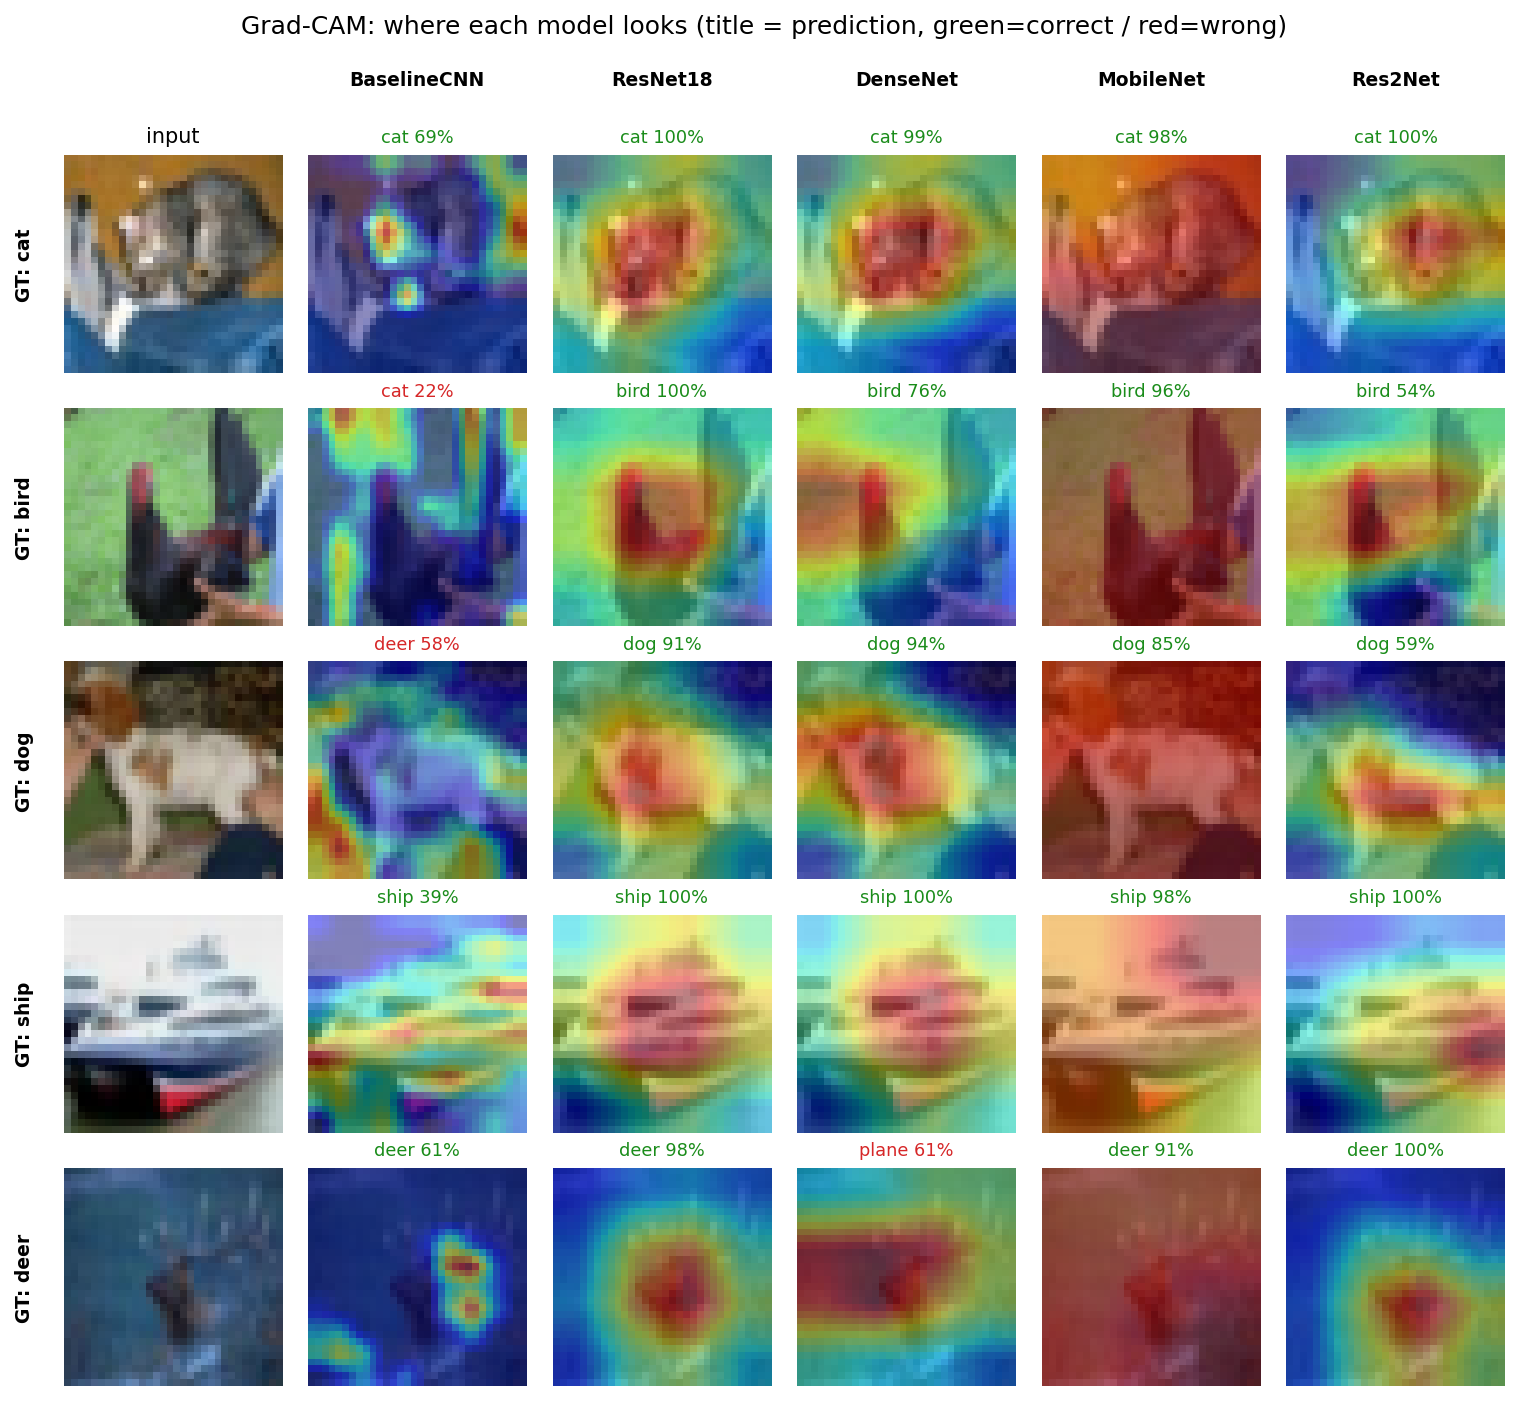
\includegraphics[width=\textwidth]{exp1_gradcam.png}
  \caption{Grad-CAM 对比：五个模型在同一批测试图上的类激活图（标题为各自预测，绿=正确/红=错误）。基线 CNN 关注弥散、易错；带跳跃/密集连接者聚焦目标、更准。}
  \label{fig:gradcam}
\end{figure}

\section{结果分析：四种网络训练过程的差异}
\begin{itemize}
  \item \textbf{无跳跃连接的 CNN（基线）.} 结构最浅、无 BatchNorm、参数仅 0.06\,M。梯度需逐层穿过普通堆叠卷积，缺乏归一化导致优化困难，损失下降最慢、准确率天花板最低（约 68.7\%），且各类别表现极不均衡。它说明：在没有残差/归一化等机制时，单纯堆叠卷积难以高效训练。
  \item \textbf{ResNet.} 残差连接 $y=F(x)+x$ 与 BatchNorm 共同作用，提供了梯度直通路径，\textbf{收敛最快、训练最稳定}，30 个 epoch 即达到 89.8\%，训练损失降到 0.12，曲线平滑无明显波动。
  \item \textbf{DenseNet.} 密集拼接带来强特征复用，使其以\textbf{最少的参数（0.246\,M）}获得 87.4\% 的高精度，参数效率冠军；每层直连损失，梯度流动顺畅。但收敛速度略慢于 ResNet，且通道拼接使显存占用偏高。
  \item \textbf{MobileNet.} 深度可分离卷积大幅降低参数与计算量（3.22\,M），单位轮次训练快、总耗时最短；但由于缺少残差且表达能力受限，收敛相对较慢、最终精度（84.6\%）略低于 ResNet/DenseNet，是\textbf{精度与效率的折中}。
\end{itemize}

\textbf{梯度流动的直接证据.} 上述差异的根源可由“初始化时梯度沿深度的传播”直接观察到。由于老师的基线 CNN 仅 5 层、深度不足以暴露深层梯度问题，我们采用 ResNet 论文式的\textbf{同深度对照}：在同为 18 层的网络上分别开关 BatchNorm 与跳跃连接，对一个 batch 做一次反向传播，记录各卷积层权重梯度的幅值（图~\ref{fig:gradflow}）。可见：(1) \textbf{无 BN、无跳跃}的普通深层网络梯度在靠近输入端急剧衰减，最浅层梯度仅约为最深层的 $10^{-4}$（梯度消失），底层几乎无法学习；(2) 仅加入 \textbf{BatchNorm} 即可把梯度均匀度提升约两个数量级，是缓解初始化期梯度消失的首要因素；(3) 在此之上，\textbf{跳跃连接（ResNet）与密集连接（DenseNet）}进一步使各层梯度更均匀（DenseNet 最高），且随深度增加其作用愈发关键。这解释了带 BN 与跳跃/密集连接的四个网络为何能稳定快速收敛；也说明基线 CNN 的瓶颈主要来自\textbf{容量小与缺少归一化}，而非其自身深度的梯度消失。

\begin{figure}[H]
  \centering
  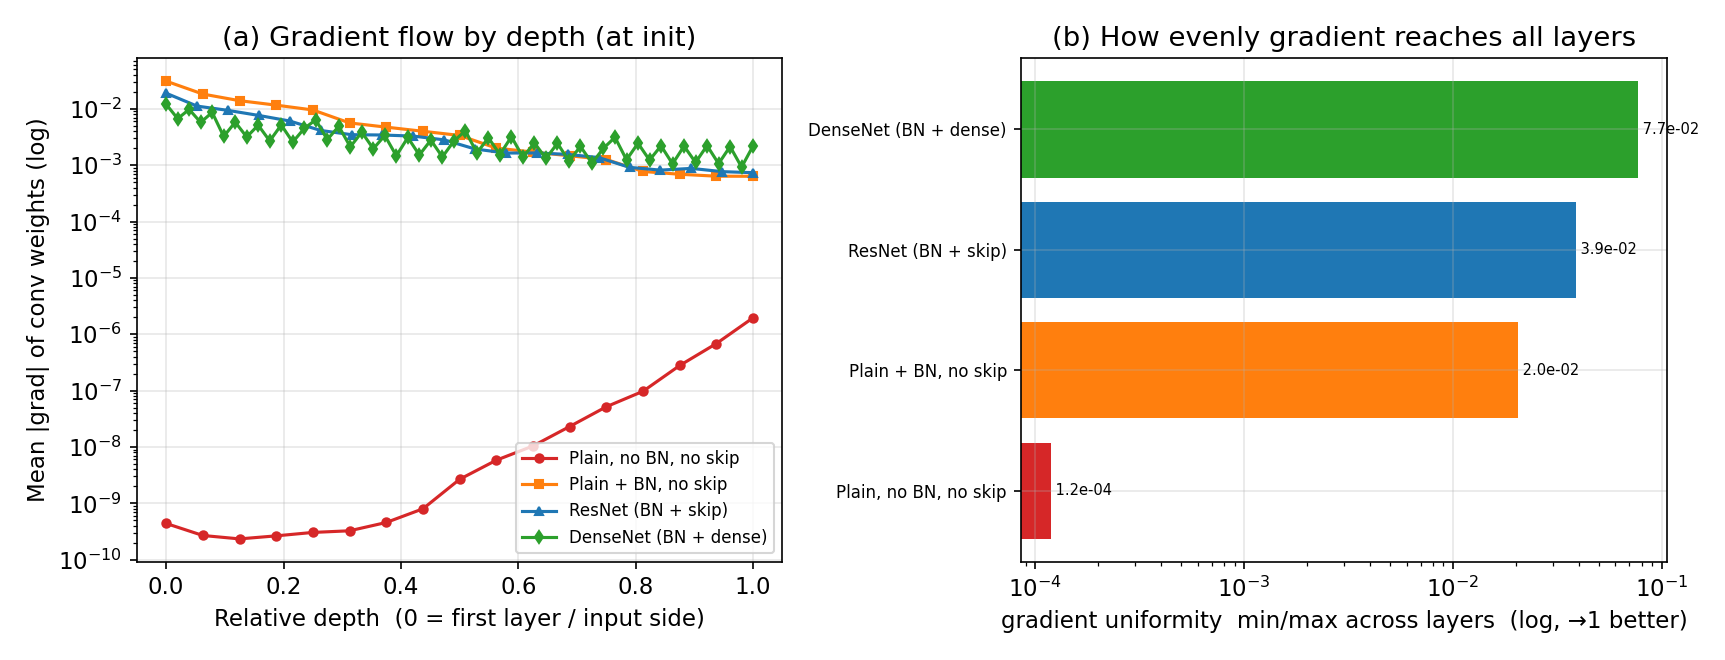
\includegraphics[width=\textwidth]{exp1_gradflow.png}
  \caption{初始化时逐层梯度幅值（同 18 层深度下隔离 BatchNorm 与跳跃连接）。左：梯度随相对深度的变化（对数纵轴），无 BN 无跳跃者在浅层急剧消失；右：梯度均匀度（各层 min/max，越接近 1 越好）。}
  \label{fig:gradflow}
\end{figure}

\textbf{收敛速度与计算效率.} 再从“达到目标精度所需 epoch”和“计算量—精度”两个角度量化训练差异（图~\ref{fig:eff}）。ResNet/Res2Net 仅 5--6 个 epoch 即达到 80\% 测试精度，DenseNet 约 8 个、MobileNet 约 14 个，而基线 CNN 始终无法达到；在“计算量 vs 精度”平面上，DenseNet 以最少参数与较低 FLOPs 取得 87\% 精度、位于效率前沿，MobileNet 计算量最低，Res2Net 精度最高但 FLOPs 也最大（约为 ResNet 的 1.4 倍）。

\begin{figure}[H]
  \centering
  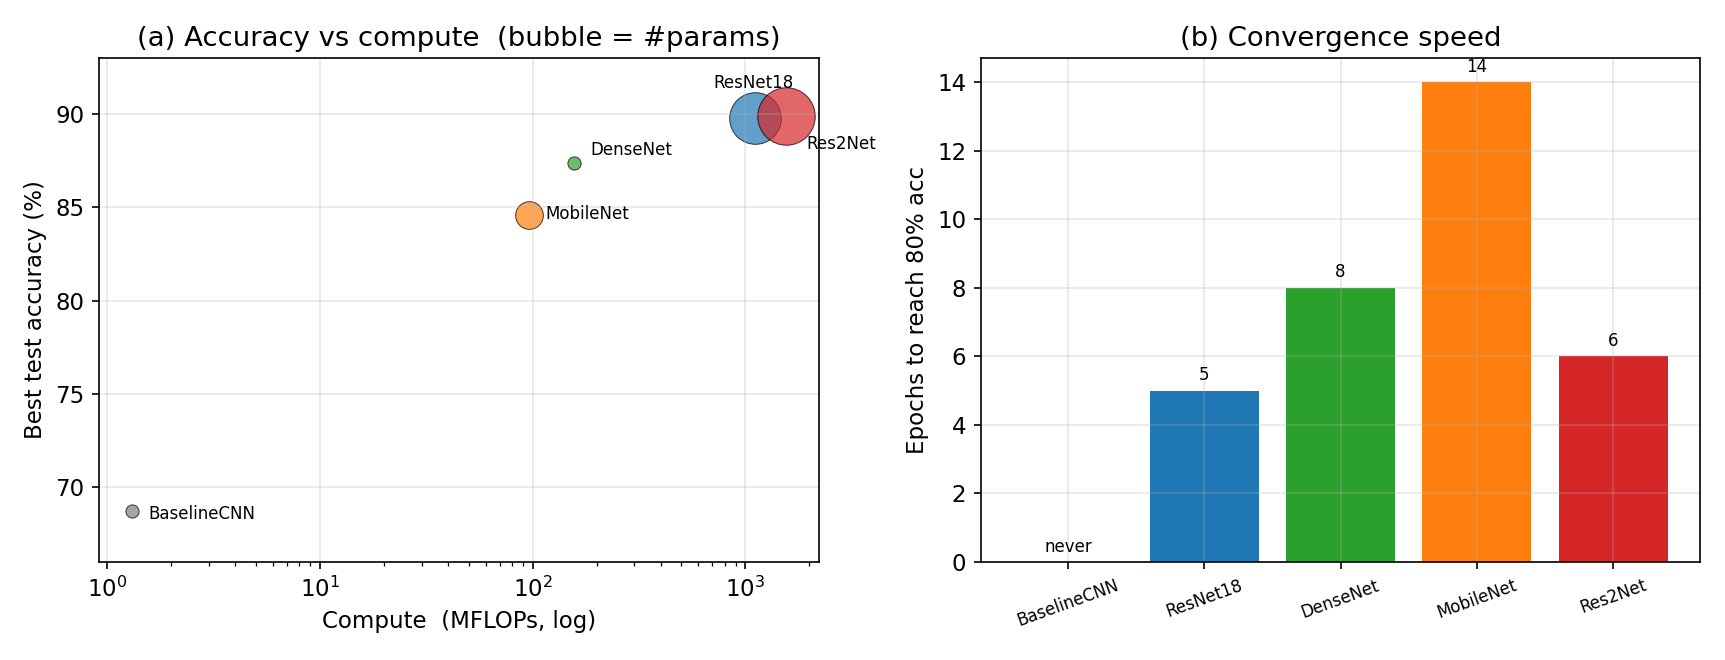
\includegraphics[width=\textwidth]{exp1_efficiency.png}
  \caption{左：计算量（MFLOPs，对数轴）与最佳准确率，气泡大小表示参数量；右：达到 80\% 测试准确率所需的 epoch 数（收敛速度，基线 CNN 始终未达标）。}
  \label{fig:eff}
\end{figure}

综合来看，跳跃连接（ResNet）与密集连接（DenseNet）显著改善了梯度传播与收敛行为，是相对基线 CNN 提升最关键的因素；MobileNet 则在牺牲少量精度的前提下换取了轻量化。

\section{扩展：Res2Net 的优势与劣势}
\textbf{优势.} Res2Net 在模块内构造多尺度感受野，获得了\textbf{全场最高的总体准确率（89.92\%）}，并在最难的 \texttt{cat} 类上达到 84.1\%、显著优于同级 ResNet 的 73.3\%，说明多尺度表达对多尺度/难样本确有帮助。

\textbf{劣势.} 其代价是\textbf{参数量最大（13.84\,M）、训练最慢（45.5\,min，约为 ResNet 的两倍）}；而在 CIFAR-10 这种低分辨率任务上，其总体精度相比 ResNet 仅高出约 0.1 个百分点，边际收益有限。可以预期，Res2Net 的多尺度优势在更高分辨率或目标检测/分割等任务上会更加明显。

\textbf{逐类视角：性能的“重分配”.} 把 Res2Net 与 ResNet 的逐类准确率做差（图~\ref{fig:res2net}）可以看到，二者的差异并非“全面变好”，而更像一次性能的\textbf{重分配}：Res2Net 在最难的 \texttt{cat}（$+10.8$ 个百分点）、\texttt{frog}、\texttt{plane} 等类别上明显提升，却在 \texttt{horse}（$-7.4$）、\texttt{bird} 等类别上有所下降，整体仅净增约 $0.1$ 个百分点。这与“多尺度感受野改变了模型所擅长的样本类型”相吻合，正是其“优势与劣势并存”的直观体现；同时也提示：单次训练得到的逐类波动应结合多次实验谨慎解读。

\begin{figure}[H]
  \centering
  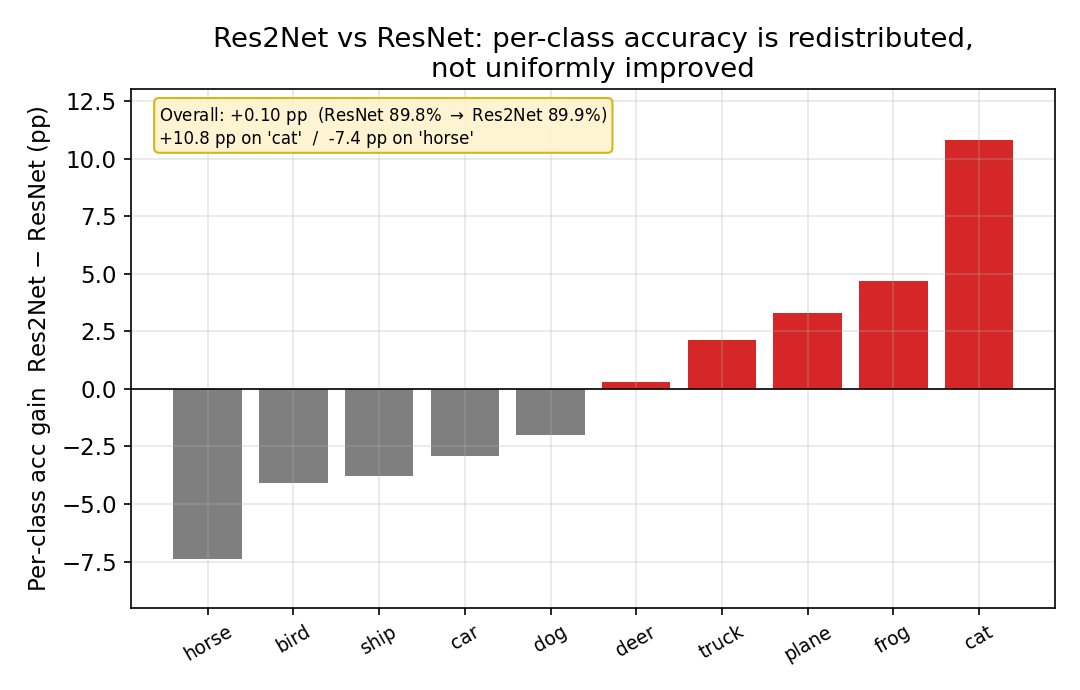
\includegraphics[width=0.78\textwidth]{exp1_res2net.png}
  \caption{Res2Net 与 ResNet 的逐类准确率之差（红=Res2Net 更高）。整体净增仅约 0.1 个百分点，但在难类 \texttt{cat} 上 $+10.8$、在 \texttt{horse} 上 $-7.4$，呈现“重分配”而非一致提升。}
  \label{fig:res2net}
\end{figure}

\section{结论}
在统一训练协议下对五个网络的对比表明：
\begin{enumerate}
  \item 残差/密集连接是相对无跳连基线 CNN（68.7\%）实现大幅提升的关键，ResNet 由 68.7\% 提升至 89.8\%；
  \item \textbf{ResNet} 综合性价比最佳（高精度、中等开销、收敛快稳）；\textbf{DenseNet} 参数效率最高（0.25\,M 达 87.4\%）；\textbf{MobileNet} 适合轻量化部署；\textbf{Res2Net} 精度最高、对难样本最稳，但开销最大；
  \item 模型选择应结合精度、参数量、训练成本与部署约束综合权衡。
\end{enumerate}

\begin{thebibliography}{9}
  \bibitem{resnet} K.~He, X.~Zhang, S.~Ren, J.~Sun. Deep Residual Learning for Image Recognition. \textit{CVPR}, 2016.
  \bibitem{densenet} G.~Huang, Z.~Liu, L.~van der Maaten, K.~Q.~Weinberger. Densely Connected Convolutional Networks. \textit{CVPR}, 2017.
  \bibitem{mobilenet} A.~G.~Howard et al. MobileNets: Efficient Convolutional Neural Networks for Mobile Vision Applications. \textit{arXiv:1704.04861}, 2017.
  \bibitem{res2net} S.~Gao, M.~Cheng, K.~Zhao, X.~Zhang, M.~Yang, P.~Torr. Res2Net: A New Multi-scale Backbone Architecture. \textit{IEEE TPAMI}, 2021.
\end{thebibliography}

\end{document}
